\documentclass[10pt,xcolor={dvipsnames},fleqn]{beamer}
%\documentclass[handout,10pt,xcolor={dvipsnames},fleqn]{beamer}
\usepackage{isse}


\usepackage{apalike}
\usepackage[utf8]{inputenc}
\usepackage{pdfpages}
%\usepackage{ngerman}
\usepackage{stmaryrd,amsmath,amssymb}
\usepackage{color}
\usepackage{enumerate}
\usepackage[makeroom]{cancel}
\usepackage{mdframed}
\usepackage{xskak}
\usepackage{marvosym}
\setchessboard{showmover=false}
\usepackage[noend]{algpseudocode}   % package for algorithms
\usepackage{algorithm}
\usepackage{tikz}

\usepackage[absolute,overlay]{textpos}

\usetikzlibrary{trees,calc,shapes,arrows,matrix,shadows,decorations.markings}

\mdfdefinestyle{theoremstyle}{
linecolor=red,linewidth=2pt,
frametitlerule=true,
frametitlebackgroundcolor=gray!20,
innertopmargin=\topskip,
}
\definecolor{LRed}{rgb}{1,.8,.8}
\definecolor{MRed}{rgb}{1,.6,.6}
\definecolor{HRed}{rgb}{1,.2,.2}

\usepackage{listings}
\lstdefinelanguage{mzn}
{
	morekeywords={var,int,solve,not,search,satisfy,endif,maximize,minimize,float,constraint,sum,forall,exists,array,of,include,predicate,then,commit,post,set,function,if,else,repeat,next,ann,break},
	sensitive=false,
	morecomment=[l]{\%},
	morecomment=[s]{/*}{*/},
	morestring=[b]",
}

\definecolor{lightlightgray}{gray}{0.95}
\definecolor{forestgreen}{HTML}{009B55}
\definecolor{thermicred}{rgb}{0.82, 0.1, 0.26}
\lstset
{
	basicstyle=\ttfamily\small,
	commentstyle=\ttfamily\color{thermicred},
	stringstyle=\ttfamily\color{isseorange},
	keywordstyle=\ttfamily\color{blue},
	tabsize=2,
	showstringspaces=false,
	flexiblecolumns=true,
	captionpos=b,	
	backgroundcolor=\color{lightlightgray},
	frame=single,
	 xleftmargin=\parindent,
}

\lstset{language=mzn}
\interfootnotelinepenalty=10000

% ====== custom commands

\newcommand{\prosumer}[1]{\ensuremath{\mathtt{#1}}}
% Soft Constraint Example
\newcommand{\constraintName}[1]{\ensuremath{\mathtt{#1}}}
% Biogas Constraints
\newcommand{\biogas}{biogas}
\newcommand{\biogasShort}{bio}
\newcommand{\gasFull}{\ensuremath{\constraintName{gasFull}_\mathtt{\biogasShort}}}
\newcommand{\ecoSweet}{\ensuremath{\constraintName{ecoSweet}_\mathtt{\biogasShort}}}
\newcommand{\onOff}{\ensuremath{\constraintName{onOff}_\mathtt{\biogasShort}}}
% Thermal Plant Constraints
\newcommand{\thermal}{thermal}
\newcommand{\thermalShort}{therm}
\newcommand{\ecoOpt}{\ensuremath{\constraintName{ecoOpt}_\mathtt{\thermalShort}}}
\newcommand{\inertia}{\ensuremath{\constraintName{inertia}_\mathtt{\thermalShort}}}
\newcommand{\ecoGood}{\ensuremath{\constraintName{ecoGood}_\mathtt{\thermalShort}}}
\newcommand{\hLevelThermal}[1]{$H_#1^\mathtt{\thermalShort}$}
% Electric Vehicle
\newcommand{\ev}{EV}
\newcommand{\limitBatteryUsage}{\ensuremath{\constraintName{limitBU}_\mathtt{\ev}}}
\newcommand{\prefBatteryLevel}{\ensuremath{\constraintName{prefBL}_\mathtt{\ev}}}
\newcommand{\earlyBird}{\ensuremath{\constraintName{earlyBird}_\mathtt{\ev}}}
% Organization
\newcommand{\org}{org}
\newcommand{\minMaxViolation}{\ensuremath{\constraintName{violation}_\mathtt{\org}}}
\newcommand{\hLevelOrg}[1]{$H_#1^\mathtt{\org}$}

\newcommand{\Variable}{X}
\newcommand{\LocalVariable}{\widehat{\Variable}}
\newcommand{\Domain}{D}
\newcommand{\Constraint}{C}
\newcommand{\ConstraintRelationship}{\mathcal{R}}

\newcommand{\valuation}{v}
\newcommand{\constraint}[1]{\mathrm{#1}}

\newcommand{\plantconstraint}[3]{  
\ifx#1b \constraint{best}[#3]
\else \ifx#1g \constraint{good}[#3]
\else \ifx#1a \constraint{acc}[#3]
\else \ifx#1d \constraint{diff}
\else \ifx#1l \constraint{low}[#3]
\else \ifx#1h \constraint{high}[#3]
\else \ifx#1o \constraint{org}[#3]
   \else
   \constraint{#1}_{#2}^{#3} 
   
   
\fi \fi \fi \fi \fi \fi \fi}
\usepackage{stmaryrd}

\providecommand{\smyth}[1]{\prec^{#1}}
\providecommand{\smytheq}[1]{\preceq^{#1}}

\providecommand{\checkfull}{\color{ForestGreen} \checkmark}
\providecommand{\checkhalf}{\color{BurntOrange} (\checkmark)}
\providecommand{\checknot}{\color{BrickRed} $x$}
% booktabs, tables 
\usepackage{booktabs}
\usepackage{tabularx}
\usepackage{longtable}
\usepackage{dcolumn}
\newcolumntype{R}{>{\raggedleft\arraybackslash}X}
\newcolumntype{d}[1]{D{.}{.}{#1} }
\newcolumntype{L}[1]{>{\raggedright\let\newline\\\arraybackslash\hspace{0pt}}m{#1}}


\newcommand{\code}[1]{\normalfont\texttt{\spaceskip=3pt\frenchspacing\def\{{\char123}\def\}{\char125}\def\^{\char94}\def\_{\char95}#1}}
\newcommand{\varit}[1]{{\frenchspacing\ensuremath{\normalfont\textsl{#1}}}}
\newcommand{\macit}[1]{{\frenchspacing\ensuremath{\normalfont\textsf{#1}}}}
\newcommand{\Eta}{\mathrm{H}}
\newcommand{\Mu}{\mathrm{M}}
\newcommand{\Nu}{\mathrm{N}}

\newcommand{\NZ}{\mathbb{N}}
\newcommand{\RZ}{\mathbb{R}}
\newcommand{\RZp}{\RZ_{\geq 0}}
\newcommand{\powerset}{\mathcal{P}}
\newcommand{\limp}{\mathrel{\Rightarrow}}
\newcommand{\compfun}{\mathbin{\circ}}
\newcommand{\isorel}{\mathrel{\cong}}
\newcommand{\restrict}[2]{{#1}\mathnormal{\upharpoonright}{#2}}
\newcommand{\natto}{\mathrel{\dot{\mathnormal{\to}}}}
\let\lbagold\lbag
\let\rbagold\rbag
\def\lbag{\mathopen{\lbagold}}
\def\rbag{\mathclose{\rbagold}}

\DeclareMathOperator{\Minop}{\mathrm{Min}}
\newcommand{\Min}[1]{\Minop^{#1}}
\DeclareMathOperator{\Maxop}{\mathrm{Max}}
\newcommand{\Max}[1]{\Maxop^{#1}}
\DeclareMathOperator{\finsets}{\mathcal{P}_{\mathrm{fin}}}
\DeclareMathOperator{\nefinsets}{\mathcal{P}_{\mathrm{fin}^+}}
%\DeclareMathOperator{\incfinsets}{\mathcal{I}_{\mathrm{fin}}}
\newcommand{\incfinsets}[1]{\mathcal{I}_{\mathrm{fin}}^{#1}}
\newcommand{\lowersubseteq}[1]{\mathrel{\subseteq_{#1}}}
\newcommand{\lowersupseteq}[1]{\mathrel{\supseteq_{#1}}}
\newcommand{\lowersubset}[1]{\mathrel{\subset_{#1}}}
\newcommand{\lowersupset}[1]{\mathrel{\supset_{#1}}}
\newcommand{\uppersubseteq}[1]{\mathrel{\subseteq^{#1}}}
\newcommand{\uppersupseteq}[1]{\mathrel{\supseteq^{#1}}}
\newcommand{\uppersubset}[1]{\mathrel{\subset^{#1}}}
\newcommand{\uppersupset}[1]{\mathrel{\supset^{#1}}}
\newcommand{\lowercup}[1]{\mathbin{\cup_{#1}}}
\newcommand{\uppercup}[1]{\mathbin{\cup^{#1}}}

\DeclareMathOperator{\finmsets}{\mathcal{M}_{\mathrm{fin}}}
\DeclareMathOperator{\nefinmsets}{\mathcal{M}_{\mathrm{fin}^+}}
\newcommand{\mcup}{\mathbin{\mathnormal{\cup}\llap{\text{\fontsize{8pt}{8pt}\selectfont$-$}}}}
\newcommand{\submseteq}{%
\mathrel{\mathchoice%
{\mathnormal{\subseteq}\llap{\text{\raisebox{0.3pt}{\fontsize{8pt}{8pt}\selectfont\rotatebox{90}{$-$}\hspace{1.8pt}}}}}%
{\mathnormal{\subseteq}\llap{\text{\raisebox{0.3pt}{\fontsize{8pt}{8pt}\selectfont\rotatebox{90}{$-$}\hspace{1.8pt}}}}}%
{\mathnormal{\subseteq}\llap{\text{\raisebox{-0.3pt}{\fontsize{5pt}{5pt}\selectfont\rotatebox{90}{$-$}\hspace{1.4pt}}}}}%
{\mathnormal{\subseteq}\llap{\text{\raisebox{-0.3pt}{\fontsize{5pt}{5pt}\selectfont\rotatebox{90}{$-$}\hspace{1.4pt}}}}}%
}}
\newcommand{\supmseteq}{\mathrel{\reflectbox{$\submseteq$}}}
\newcommand{\lowersubmseteq}[1]{\mathrel{\submseteq_{#1}}}
\newcommand{\uppersubmseteq}[1]{\mathrel{\submseteq^{#1}}}
\newcommand{\submset}{%
\mathrel{\mathchoice%
{\mathnormal{\subset}\llap{\text{\raisebox{-0.8pt}{\fontsize{8pt}{8pt}\selectfont\rotatebox{90}{$-$}\hspace{1.8pt}}}}}%
{\mathnormal{\subset}\llap{\text{\raisebox{-0.8pt}{\fontsize{8pt}{8pt}\selectfont\rotatebox{90}{$-$}\hspace{1.8pt}}}}}%
{\mathnormal{\subset}\llap{\text{\raisebox{-0.3pt}{\fontsize{7pt}{7pt}\selectfont\rotatebox{90}{$-$}\hspace{1pt}}}}}%
{\mathnormal{\subset}\llap{\text{\raisebox{-0.3pt}{\fontsize{7pt}{7pt}\selectfont\rotatebox{90}{$-$}\hspace{1pt}}}}}%
}}
\newcommand{\supmset}{\mathrel{\reflectbox{$\submset$}}}
\newcommand{\lowersubmset}[1]{\mathrel{\submset_{#1}}}
\newcommand{\uppersubmset}[1]{\mathrel{\submset^{#1}}}

\DeclareMathOperator{\collapseset}{\mathcal{C}}

\newcommand{\category}[1]{\mathrm{#1}}
\newcommand{\POcat}{\category{PO}}
\newcommand{\uSLcat}{\category{uSL}}
\newcommand{\poMoncat}{\category{poMon}}
\newcommand{\jMoncat}{\category{jMon}}
\newcommand{\mMoncat}{\category{mMon}}
\newcommand{\xMoncat}{{x}\category{Mon}}
\newcommand{\PVScat}{\category{PVS}}
\newcommand{\cSRngcat}{\category{cSRng}}
\newcommand{\DAGcat}{\category{DAG}}

\newcommand{\idfun}[1]{1_{#1}}
\newcommand{\functor}[1]{\mathit{#1}}
\DeclareMathOperator{\POfun}{\functor{PO}}
\DeclareMathOperator{\uSLfun}{\functor{uSL}}
\DeclareMathOperator{\poMonfun}{\functor{poMon}}
\DeclareMathOperator{\jMonfun}{\functor{jMon}}
\DeclareMathOperator{\mMonfun}{\functor{mMon}}
\DeclareMathOperator{\xMonfun}{\text{$x$}\functor{Mon}}
\DeclareMathOperator{\PVSfun}{\functor{PVS}}
\DeclareMathOperator{\cSRngfun}{\functor{cSRng}}
\DeclareMathOperator{\DAGfun}{\functor{DAG}}

\newcommand{\uSLfree}[1]{\uSLfun\langle#1\rangle}
\newcommand{\uSLeta}{\eta^{\uSLcat}}
\newcommand{\uSLetaat}[1]{\uSLeta_{#1}}
\newcommand{\uSLlift}[1]{{#1}^{\sharp_{\uSLcat}}}

\newcommand{\poMonfree}[1]{\poMonfun\langle#1\rangle}
\newcommand{\poMoneta}{\eta^{\poMoncat}}
\newcommand{\poMonetaat}[1]{\poMoneta_{#1}}
\newcommand{\poMonlift}[1]{{#1}^{\sharp_{\poMoncat}}}

\newcommand{\jMonfree}[1]{\jMonfun\langle#1\rangle}
\newcommand{\jMoneta}{\eta^{\jMoncat}}
\newcommand{\jMonetaat}[1]{\jMoneta_{#1}}
\newcommand{\jMonlift}[1]{{#1}^{\sharp_{\jMoncat}}}

\newcommand{\mMonfree}[1]{\mMonfun\langle#1\rangle}
\newcommand{\mMoneta}{\eta^{\mMoncat}}
\newcommand{\mMonetaat}[1]{\mMoneta_{#1}}
\newcommand{\mMonlift}[1]{{#1}^{\sharp_{\mMoncat}}}

\newcommand{\PVSfree}[1]{\PVSfun\langle#1\rangle}
\newcommand{\PVSeta}{\eta^{\PVScat}}
\newcommand{\PVSetaat}[1]{\PVSeta_{#1}}
\newcommand{\PVSlift}[1]{{#1}^{\sharp_{\PVScat}}}

\newcommand{\xMonfree}[1]{\xMonfun\langle#1\rangle}
\newcommand{\xMoneta}{\eta^{\xMoncat}}
\newcommand{\xMonetaat}[1]{\xMoneta_{#1}}
\newcommand{\xMonlift}[1]{{#1}^{\sharp_{\xMoncat}}}

\newcommand{\cSRngfree}[1]{\cSRngfun\langle#1\rangle}
\newcommand{\cSRngeta}{\eta^{\cSRngcat}}
\newcommand{\cSRngetaat}[1]{\cSRngeta_{#1}}
\newcommand{\cSRnglift}[1]{{#1}^{\sharp_{\cSRngcat}}}

\newcommand{\POfree}[1]{\POfun\langle#1\rangle}
\newcommand{\POeta}{\eta^{\POcat}}
\newcommand{\POetaat}[1]{\POeta_{#1}}
\newcommand{\POlift}[1]{{#1}^{\sharp_{\POcat}}}

\newcommand{\mtimes}[1]{\mathbin{\tilde{\cdot}_{#1}}}
\newcommand{\mplus}[1]{\mathbin{\tilde{\cup}_{#1}}}
\newcommand{\ftimes}[1]{\mathbin{\tilde{\mcup}^{#1}}}
\newcommand{\fplus}[1]{\mathbin{\tilde{\cup}_{#1}}}

\DeclareMathOperator{\scope}{\mathrm{sc}}
\DeclareMathOperator{\defdom}{\mathrm{def}}

\newcommand{\reflclos}[1]{\mathrel{(#1)^=}}
\newcommand{\transclos}[2][+]{\mathrel{(#2)^{#1}}}
\newcommand{\refltransclos}[1]{\mathrel{(#1)^*}}

\newcommand{\XPDrel}[2][\pi]{\rightsquigarrow^{#1}_{#2}}
\newcommand{\XPDreleq}[2][\pi]{\rightsquigarrow^{#1, =}_{#2}}
\newcommand{\XPDord}[2][\pi]{<^{#1}_{#2}}
\newcommand{\XPDordeq}[2][\pi]{\geq^{#1}_{#2}}
\newcommand{\XPDleq}[2][\pi]{\leq^{#1}_{#2}}
\newcommand{\XPDgeq}[2][\pi]{\geq^{#1}_{#2}}
\newcommand{\XPDw}[2][\pi]{w^{#1}_{#2}}
\newcommand{\XPDW}[2][\pi]{W^{#1}_{#2}}
\newcommand{\XPDk}[2][\pi]{k^{#1}_{#2}}

\newcommand{\SPDrel}{\XPDrel[\mathrm{SPD}]}
\newcommand{\SPDreleq}{\XPDreleq[\mathrm{SPD}]}
\newcommand{\SPDleq}{\XPDleq[\mathrm{SPD}]}
\newcommand{\SPDgeq}{\XPDgeq[\mathrm{SPD}]}
\newcommand{\SPDord}{\XPDord[\mathrm{SPD}]}
\newcommand{\SPDw}{\XPDw[\mathrm{SPD}]}
\newcommand{\SPDW}{\XPDW[\mathrm{SPD}]}
\newcommand{\DPDrel}{\XPDrel[\mathrm{DPD}]}
\newcommand{\DPDreleq}{\XPDreleq[\mathrm{DPD}]}
\newcommand{\DPDord}{\XPDord[\mathrm{DPD}]}
\newcommand{\DPDw}{\XPDw[\mathrm{DPD}]}
\newcommand{\DPDW}{\XPDW[\mathrm{DPD}]}
\newcommand{\TPDrel}{\XPDrel[\mathrm{TPD}]}
\newcommand{\TPDreleq}{\XPDreleq[\mathrm{TPD}]}
\newcommand{\TPDleq}{\XPDleq[\mathrm{TPD}]}
\newcommand{\TPDgeq}{\XPDgeq[\mathrm{TPD}]}
\newcommand{\TPDord}{\XPDord[\mathrm{TPD}]}
\newcommand{\TPDw}{\XPDw[\mathrm{TPD}]}
\newcommand{\TPDW}{\XPDW[\mathrm{TPD}]}

\DeclareMathSymbol{\UPi}{\mathalpha}{operators}{"05}



\renewcommand{\submseteq}{%
\mathrel{\mathchoice%
{\mathnormal{\subseteq}\llap{\text{\raisebox{0.0pt}{\fontsize{7.5pt}{7.5pt}\selectfont\rotatebox{90}{$-$}\hspace{1.6pt}}}}}%
{\mathnormal{\subseteq}\llap{\text{\raisebox{0.0pt}{\fontsize{7.5pt}{7.5pt}\selectfont\rotatebox{90}{$-$}\hspace{1.6pt}}}}}%
{\mathnormal{\subseteq}\llap{\text{\raisebox{-0.3pt}{\fontsize{7pt}{7pt}\selectfont\rotatebox{90}{$-$}\hspace{1pt}}}}}%
{\mathnormal{\subseteq}\llap{\text{\raisebox{-0.3pt}{\fontsize{7pt}{7pt}\selectfont\rotatebox{90}{$-$}\hspace{1pt}}}}}%
}}


\tikzset{
   main node/.style={circle,fill=black!15,draw,font=\sffamily},
   constraint node/.style={main node, circle, inner sep=2pt,font=\sffamily\small},   
   treestyle/.style={rectangle,fill=black!15,draw,font=\sffamily}
}


\mdtheorem[style=theoremstyle]{definition}{Definition}

\renewcommand{\vec}[1]{\mathbf{#1}}
\newcommand{\tupleOf}[1]{\langle #1 \rangle}
\newcommand{\cemph}[1]{\alert{#1}}
\usepackage{framed}
\usepackage{ifthen}

\usetikzlibrary{decorations.pathmorphing,calc,shadows.blur,shadings}
\usetikzlibrary{mindmap,trees,automata,arrows}
\usepackage{extrabeamercmds}

\newcommand{\hFirst}[1]{{\color{isseorange} #1}}
\newcommand{\hSecond}[1]{{\color{CornflowerBlue} #1}}

\newcounter{mathseed}
\setcounter{mathseed}{3}
\pgfmathsetseed{\arabic{mathseed}} % To have predictable results
% Define a background layer, in which the parchment shape is drawn
\pgfdeclarelayer{background}
\pgfsetlayers{background,main}


% This is the base for the fractal decoration. It takes a random point between the start and end, and
% raises it a random amount, thus transforming a segment into two, connected at that raised point
% This decoration can be applied again to each one of the resulting segments and so on, in a similar
% way of a Koch snowflake.
\pgfdeclaredecoration{irregular fractal line}{init}
{
  \state{init}[width=\pgfdecoratedinputsegmentremainingdistance]
  {
    \pgfpathlineto{\pgfpoint{random*\pgfdecoratedinputsegmentremainingdistance}{(random*\pgfdecorationsegmentamplitude-0.02)*\pgfdecoratedinputsegmentremainingdistance}}
    \pgfpathlineto{\pgfpoint{\pgfdecoratedinputsegmentremainingdistance}{0pt}}
  }
}


% define some styles
\tikzset{
   paper/.style={draw=black!10, blur shadow, every shadow/.style={opacity=1, black}, 
                 lower left=black!10, upper left=black!5, upper right=white, lower right=black!5, fill=none},
   irregular cloudy border/.style={decoration={irregular fractal line, amplitude=0.2},
           decorate,
     },
   irregular spiky border/.style={decoration={irregular fractal line, amplitude=-0.2},
           decorate,
     },
   ragged border/.style={ decoration={random steps, segment length=7mm, amplitude=2mm},
           decorate,
   }
}

\tikzset{
  normal border/.style={orange!30!black!10, decorate, 
     decoration={random steps, segment length=2.5cm, amplitude=.7mm}},
  torn border/.style={orange!30!black!5, decorate, 
     decoration={random steps, segment length=.5cm, amplitude=1.7mm}}}


\def\tornpaper#1{%
\ifthenelse{\isodd{\value{mathseed}}}{%
\tikz{
  \node[inner sep=1em] (A) {#1};  % Draw the text of the node
  \begin{pgfonlayer}{background}  % Draw the shape behind
  \fill[paper] % recursively decorate the bottom border
     \pgfextra{\pgfmathsetseed{\arabic{mathseed}}\addtocounter{mathseed}{1}}%
      {decorate[irregular cloudy border]{decorate{decorate{decorate{decorate[ragged border]{
        (A.north west) -- (A.north east)
      }}}}}}
      -- (A.south east)
     \pgfextra{\pgfmathsetseed{\arabic{mathseed}}}%
      {decorate[irregular spiky border]{decorate{decorate{decorate{decorate[ragged border]{
      -- (A.south west)
      }}}}}}
      -- (A.north west);
  \end{pgfonlayer}}
}{%
\tikz{
  \node[inner sep=1em] (A) {#1};  % Draw the text of the node
  \begin{pgfonlayer}{background}  % Draw the shape behind
  \fill[paper] % recursively decorate the bottom border
     \pgfextra{\pgfmathsetseed{\arabic{mathseed}}\addtocounter{mathseed}{1}}%
      {decorate[irregular spiky border]{decorate{decorate{decorate{decorate[ragged border]{
        (A.north east) -- (A.north west)
      }}}}}}
      -- (A.south west)
     \pgfextra{\pgfmathsetseed{\arabic{mathseed}}}%
      {decorate[irregular cloudy border]{decorate{decorate{decorate{decorate[ragged border]{
      -- (A.south east)
      }}}}}}
      -- (A.north east);
  \end{pgfonlayer}}
}}


% Macro to draw the shape behind the text, when it fits completly in the
% page
\def\parchmentframe#1{
\tikz{
  \node[inner sep=2em] (A) {#1};  % Draw the text of the node
  \begin{pgfonlayer}{background}  % Draw the shape behind
  \fill[normal border] 
        (A.south east) -- (A.south west) -- 
        (A.north west) -- (A.north east) -- cycle;
  \end{pgfonlayer}}}

% Macro to draw the shape, when the text will continue in next page
\def\parchmentframetop#1{
\tikz{
  \node[inner sep=2em] (A) {#1};    % Draw the text of the node
  \begin{pgfonlayer}{background}    
  \fill[normal border]              % Draw the ``complete shape'' behind
        (A.south east) -- (A.south west) -- 
        (A.north west) -- (A.north east) -- cycle;
  \fill[torn border]                % Add the torn lower border
        ($(A.south east)-(0,.2)$) -- ($(A.south west)-(0,.2)$) -- 
        ($(A.south west)+(0,.2)$) -- ($(A.south east)+(0,.2)$) -- cycle;
  \end{pgfonlayer}}}

% Macro to draw the shape, when the text continues from previous page
\def\parchmentframebottom#1{
\tikz{
  \node[inner sep=2em] (A) {#1};   % Draw the text of the node
  \begin{pgfonlayer}{background}   
  \fill[normal border]             % Draw the ``complete shape'' behind
        (A.south east) -- (A.south west) -- 
        (A.north west) -- (A.north east) -- cycle;
  \fill[torn border]               % Add the torn upper border
        ($(A.north east)-(0,.2)$) -- ($(A.north west)-(0,.2)$) -- 
        ($(A.north west)+(0,.2)$) -- ($(A.north east)+(0,.2)$) -- cycle;
  \end{pgfonlayer}}}

% Macro to draw the shape, when both the text continues from previous page
% and it will continue in next page
\def\parchmentframemiddle#1{
\tikz{
  \node[inner sep=2em] (A) {#1};   % Draw the text of the node
  \begin{pgfonlayer}{background}   
  \fill[normal border]             % Draw the ``complete shape'' behind
        (A.south east) -- (A.south west) -- 
        (A.north west) -- (A.north east) -- cycle;
  \fill[torn border]               % Add the torn lower border
        ($(A.south east)-(0,.2)$) -- ($(A.south west)-(0,.2)$) -- 
        ($(A.south west)+(0,.2)$) -- ($(A.south east)+(0,.2)$) -- cycle;
  \fill[torn border]               % Add the torn upper border
        ($(A.north east)-(0,.2)$) -- ($(A.north west)-(0,.2)$) -- 
        ($(A.north west)+(0,.2)$) -- ($(A.north east)+(0,.2)$) -- cycle;
  \end{pgfonlayer}}}

% Define the environment which puts the frame
% In this case, the environment also accepts an argument with an optional
% title (which defaults to ``Example'', which is typeset in a box overlaid
% on the top border
\newenvironment{parchment}[1][Example]{%
  \def\FrameCommand{\parchmentframe}%
  \def\FirstFrameCommand{\parchmentframetop}%
  \def\LastFrameCommand{\parchmentframebottom}%
  \def\MidFrameCommand{\parchmentframemiddle}%
  \vskip\baselineskip
  \MakeFramed {\FrameRestore}
  \noindent\tikz\node[inner sep=1ex, draw=black!20,fill=white, 
          anchor=west, overlay] at (0em, 2em) {\sffamily#1};\par}%
{\endMakeFramed}


\title{Constraint Relationships in MiniZinc}
\author{Case Studies}

\date{\today}

\begin{document}

\titleframe


\begin{frame}
\frametitle{Preferences in Constraint Solving}

Constraint problem $(X, D, C)$ 
\begin{itemize}
  \item \cemph{Variables} $X$,
\cemph{Domains} $D = (D_x)_{x \in X}$,
\cemph{Constraints} $C$
\end{itemize}

\vspace*{1ex}

How to deal with \cemph{over-constrained} problems?

\vspace*{2ex}

$((\{ \mathrm{x}, \mathrm{y}, \mathrm{z} \},
\mathrm{D}_{\mathrm{x}} = \mathrm{D}_{\mathrm{y}} =
\mathrm{D}_{\mathrm{z}} = \{ 1, 2, 3 \}), \{ \mathrm{c}_1,
\mathrm{c}_2, \mathrm{c}_3 \})$ mit 
\bgroup\abovedisplayskip4pt\belowdisplayskip4pt
\begin{align*}
  \mathrm{c}_1 &: \mathrm{x} + 1 = \mathrm{y}
\\[-.4ex]
  \mathrm{c}_2 &: \mathrm{z} = \mathrm{y} + 2
\\[-.4ex]
  \mathrm{c}_3 &: \mathrm{x} + \mathrm{y} \leq 3
\end{align*}
\egroup

\begin{itemize}
  \item Not all constraints can be satisfied simultaneously
\begin{itemize} \pause
  \item e.\,g., $\mathrm{c}_2$ forces $\mathrm{z} = 3$ and $\mathrm{y} = 1$, conflicting $\mathrm{c}_1$
\end{itemize}

  \item We can \cemph{choose} between assignments satisfying $\{ \mathrm{c}_1, \mathrm{c}_3 \}$ or $\{ \mathrm{c}_2, \mathrm{c}_3 \}$.
\end{itemize}

\vspace*{2ex}

Which assignments $v \in [X \to D]$ should be \alert{preferred} by an agent/several agents?

\end{frame}

\begin{frame}
\frametitle{Constraint Relationships}

Approach~\cite{Schiendorfer13}
\begin{itemize}
  \item Define relation $R$ over constraints $C$ to denote which constraints are more important than others, e.\,g.
\begin{itemize}
  \item $\mathrm{c}_1$ is more important than  $\mathrm{c}_2$

  \item $\mathrm{c}_1$ is more important than $\mathrm{c}_3$
\end{itemize}
\end{itemize}
\begin{textblock*}{2.5cm}[1,1](\textwidth-1.5cm,\textheight-4.03cm)
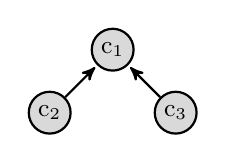
\begin{tikzpicture}[auto,
                    ->,>=stealth',shorten >=1pt,thick,
                    node distance=.7cm,inner sep=2pt,
                    constraint/.style={circle,fill=black!15,draw,font=\sffamily\small}]
\node[constraint node] (1) at (0, 0)                   {$\mathrm{c}_1$};
\node[constraint node] (2) at ($ (1) + (-0.8, -0.8) $) {$\mathrm{c}_2$};  
\node[constraint node] (3) at ($ (1) + ( 0.8, -0.8) $) {$\mathrm{c}_3$};  
%  
\path[every node/.style={font=\sffamily\tiny}]
  (2) edge (1)
  (3) edge (1)
  ;
\end{tikzpicture}
\end{textblock*}

\vspace*{5.6ex}

Benefits
\begin{itemize}
  \item \cemph{Qualitative} formalism --- easy to specify
  \item Graphical interpretation 
\begin{itemize}
 \item Semantics (\alert{how} much more important is a constraint) regulated by 
  \item \cemph{dominance properties} that are either ``hierarchical'' or ``egalitarian''
  \item Single-Predecessors-Dominance (SPD) vs. Transitive-Predecessors-Dominance (TPD)
\end{itemize}

\end{itemize}

%\vspace*{2ex}
%\begin{small}
%A.~Schiendorfer, J.-Ph.~Steghöfer, A.~Knapp, F.~Nafz, W.~Reif (2013)
%\end{small}
\end{frame}


\begin{frame}[fragile]{SoftConstraints in MiniZinc}
\begin{lstlisting}
% X: {x,y,z} D_i = {1,2,3}, i in X
%    * c1: x + 1 = y   * c2: z = y + 2 * c3: x + y <= 3
% (c) ISSE
% isse.uni-augsburg.de/en/software/constraint-relationships/
include "soft_constraints/minizinc_bundle.mzn";

var 1..3: x; var 1..3: y; var 1..3: z;

% read as "soft constraint c1 is satisfied iff x + 1 = y"
constraint x + 1 = y <-> satisfied[1];
constraint z = y + 2 <-> satisfied[2];
constraint x + y <= 3 <-> satisfied[3];

% soft constraint specific for this model
nScs = 3; nCrEdges = 2;
crEdges = [| 2, 1 | 3, 1 |]; % read c2 is less important than c1

solve minimize penSum; % minimize the sum of penalties
\end{lstlisting}

\end{frame}


\begin{frame}{Case Studies}
Applied to domains where 
\begin{itemize}
\item Certain properties should really capture \alert{preferences}, not constraints
\item at design time, it is \alert{unclear} whether an instance is actually solvable
\item Solution space is \emph{combinatorial}
\begin{itemize}
\item[-] Discrete choices
\item[-] Additional hard constraints
\end{itemize}
\end{itemize}

\vspace*{2ex}

Illustrative case studies (found in \texttt{example-problems})
\begin{itemize}
\item Mentor Matching
\item Exam Scheduling
\item Power Plant Scheduling
\end{itemize}
\end{frame}


\begin{frame}[fragile]{Mentor Matching}

\textbf{Goal}: Assign mentees (e.g. students) to mentors (e.g. companies) such that 
\begin{itemize}
\item Students are most satisfied with their mentors 
\item Companies are satisfied with their mentees
\item Two-sided preferences
\end{itemize}

\vspace*{2ex}

So far, sounds like a typical \emph{stable matching} problem, but:

\begin{itemize}
\item We do not have a 1:1 mapping (companies advise several students)
\item Additional constraints are present
\begin{itemize}
\item[-] Each company has to advise at least $l$, at most $u$ students
\item[-] The number of advised students \emph{should} be roughly equal per company (fairness)
\item[-] Students actually despising a company should not be forced to go there (\emph{hard exclusion} of solutions)
\end{itemize}
\end{itemize}
\end{frame}


\begin{frame}[fragile]{Mentor Matching: Example}
\begin{center}
\tikzset{onslide/.code args={<#1>#2}{%
  \only<#1>{\pgfkeysalso{#2}}
}}

\tikzstyle{highlight}=[isseorange,ultra thick]
\tikzstyle{highlight2}=[CornflowerBlue,ultra thick,rounded corners]
\tikzstyle{defaultStyle}=[white,ultra thick,rounded corners]

\tikzstyle{impo}=[dashed]
\begin{tikzpicture}[every node/.style={
anchor=base,
%text depth=.5ex,
%text height=2ex,
%minimum height=2ex,
align=center,
rectangle,
text width=2em
}]
\matrix (magic) [nodes in empty cells, ampersand replacement=\&,row sep=0.4cm,column sep=1.5cm]
{
\node[draw,defaultStyle, onslide={<3->{highlight2}}](s1){\includegraphics[width=\textwidth]{img/businessman.png}}; \& \& \& \node[text width=4em, defaultStyle, draw, onslide={<3->{highlight2}}](c1) {\includegraphics[width=\textwidth]{img/airplane.png}}; \\
\node(s2){\includegraphics[width=\textwidth]{img/woman.png}};       \& \& \& \node(c2) {\includegraphics[width=2\textwidth]{img/logistics.png}}; \\
\node(s3){\includegraphics[width=\textwidth]{img/man.png}};         \& \& \& \node(c3) {\includegraphics[width=2\textwidth]{img/enrgy.png}}; \\
\node[defaultStyle, draw, onslide={<3->{highlight2}}](s4){\includegraphics[width=\textwidth]{img/woman2.png}};      \& \\
};

\draw[onslide={<2->{highlight}}] (s1) -- (c1);
\draw[] (s1) -- (c2);

\draw[onslide={<2->{highlight}}] (s2) -- (c1);
\draw[] (s2) -- (c3);

\draw[onslide={<2->{highlight}}] (s3) -- (c2);

\draw[onslide={<2->{highlight}}] (s4) -- (c3);
\draw[] (s4) -- (c2);
%
%\draw[onslide={<1-2>{highlight}}] (z) -- (3);
%\draw[onslide={<3>{highlight}}] (z) -- (2);
%
%\draw[onslide={<1-2>{highlight}}] (t) -- (2);
%\draw[] (t) -- (1);
%\draw[onslide={<3>{highlight}}] (t) -- (5);
%\draw[] (t) -- (3);
%\draw[] (t) -- (4);
%\draw[onslide={<1>{highlight}}] (u) -- (4);
%\draw[] (u) -- (3);
%\draw[] (u) -- (5);
%\draw[] (u) -- (6);
\end{tikzpicture}
\end{center}
\onslide<2->{This \alert{assignment} respects the students' preferences (edges) \onslide<3->{but ignores the {\color{CornflowerBlue} companies' preferences}.}}
\onslide<4->{\tiny ok, it's not really a \emph{matching} since companies supervise more than one student \ldots }
\end{frame}

\begin{frame}[fragile]{Mentor Matching: Model}
\begin{lstlisting}
int: n; set of int: STUDENT = 1..n;
int: m; set of int: COMPANY = 1..m;

% assign students to companies
array[STUDENT] of var COMPANY: worksAt;

% insert relationships of students and companies here

int: minPerCompany = 2; int: maxPerCompany = 3;
constraint global_cardinality_low_up ( 
           worksAt, [c | c in COMPANY], 
           [minPerCompany | c in COMPANY], 
           [maxPerCompany | c in COMPANY]); 
           
solve 
:: int_search([ satisfied[mostImpFirst[i]] | i in SOFTCONSTRAINTS], 
  input_order, indomain_max, complete)
minimize penSum;
\end{lstlisting}
\end{frame}

\begin{frame}[fragile]{Mentor Matching: Preferences}
\begin{lstlisting}
n = 3; m = 3;
int: brenner = 1;
int: teufel = 2;
int: fennek  = 3;

int: cupgainini = 1;
int: gsm = 2;
int: junedied = 3;

% specify soft constraints, order by relationship
constraint worksAt[teufel] = junedied <-> satisfied[teufJune];
constraint worksAt[teufel] = cupgainini <-> satisfied[teufCap];
constraint worksAt[teufel] = gsm <-> satisfied[teufGsm];

constraint worksAt[fennek ] in {cupgainini, gsm}  <-> satisfied[fenFavs];
constraint worksAt[fennek ] in {junedied} <-> satisfied[fenOK];

crEdges = [| teufGsm, teufCap | teufGsm, teufJune 
            | fenOK, fenFavs |];
\end{lstlisting}
\end{frame}

\begin{frame}[fragile]{Mentor Matching: Refinements}
Split company and student preferences:
\begin{lstlisting}
% first, our students' preferences
var int: penStud = sum(sc in 1..lastStudentPref) 
     (bool2int(not satisfied[sc]) * penalties[sc]);
% now companies' preferences
var int: penComp = sum(sc in lastStudentPref+1..nScs)
     (bool2int(not satisfied[sc]) * penalties[sc]);
\end{lstlisting}

\vspace*{3ex}

Optimize lexicographically

\begin{lstlisting}
solve 
:: int_search([ satisfied[mostImpFirst[i]] | i in SOFTCONSTRAINTS],%... 
%search minimize_lex([penStud, penComp]) /\ if % ...
search minimize_lex([penComp, penStud]) /\ if % ...
\end{lstlisting}
\end{frame}

\begin{frame}[fragile]{Mentor Matching: Priority Example}
Taken from example: \texttt{student-company-matching.mzn}
\begin{lstlisting}
solve 
:: int_search([ satisfied[mostImpFirst[i]] | i in SOFTCONSTRAINTS],%... 
search minimize_lex([penStud, penComp]) /\ if %...
\end{lstlisting}

\small
\begin{verbatim}
worksAt = [1, 3, 2, 3], penalty Students: 8, penalty Companies: 6
----------
==========
\end{verbatim}

\begin{lstlisting}
solve 
:: int_search([ satisfied[mostImpFirst[i]] | i in SOFTCONSTRAINTS],%... 
search minimize_lex([penStud, penComp]) /\ if %...
\end{lstlisting}

\small
\begin{verbatim}
worksAt = [1, 3, 1, 2], penalty Students: 10, penalty Companies: 4
----------
==========
\end{verbatim}
Here, company 1 (cupgainini) wanted to have student 3, and company 2 (APS) did not have any preferences whatsoever (so accepted student 4 instead of 3). Student 4 would have liked company 3 (junedied) better, though.
\end{frame}

\begin{frame}[fragile]{Mentor Matching: Real Instance}
\begin{itemize}
\item Collected data from winter term

\begin{parchment}
\begin{verbatim}
"the favorites":
1. JuneDied-Lynx- HumanIT
2. Cupgainini
 
"I could live with that":
3. Seamless-German
4. gsm systems
5. Yiehlke
 
"I think, we won't be happy":
6. APS
7. Delphi Databases
\end{verbatim} 
\end{parchment}
\end{itemize}
\end{frame}

\begin{frame}[fragile]{Mentor Matching: Real Instance}
\begin{itemize}
\item Gave precedence to \alert{students}
\begin{itemize}
\item[-] After all, what should companies do with unhappy students?
\end{itemize}
\item Search space: 7 companies for 16 students $\rightarrow 7^{16} = 3.3233 \cdot 10^{13}$
\vspace*{2ex}
\item Led to a constraint problem with 
\begin{itemize}
\item[-] 77 student preferences (soft constraints) from 16 students
\item[-] of a total of 114 soft constraints (37 company preferences) 
\end{itemize}

\vspace*{2ex}

\item \emph{Proved} optimal solution 
\begin{itemize}
\item[-] 4 minutes compilation 
\item[-] another 2m 12s solving time
\end{itemize}
\end{itemize}
\end{frame}


\begin{frame}[fragile]{Exam Scheduling}

\textbf{Goal}: Assign exam dates to students such that 
\begin{itemize}
\item Each student likes their appoints (\emph{approves of it})
\item The number of distinct dates is minimized (to reduce time investment of teachers)
\end{itemize}

%\vspace*{2ex}
%\begin{parchment}
\begin{center}
\includegraphics[width=.15\textwidth]{img/voting.png}
\hspace*{4ex}
\includegraphics[width=.5\textwidth]{img/Voting.pdf}
\end{center}
%\end{parchment}

\begin{itemize}
\item No preference of any student should be weighted higher than another one's
\item Solution (exam schedule) is a shared decision

\end{itemize}
\end{frame}

\begin{frame}[fragile]{Exam Scheduling: Core Model}
See \texttt{exam-scheduling-approval.mzn}:
\begin{lstlisting}
% Exam scheduling example with just a set of 
% approved dates and *impossible* ones
include "globals.mzn";
include "soft_constraints/soft_constraints.mzn";

int: n; set of int: STUDENT = 1..n; 
int: m; set of int: DATE = 1..m;
array[STUDENT] of set of DATE: possibles;
array[STUDENT] of set of DATE: impossibles;

% the actual decisions
array[STUDENT] of var DATE: scheduled;

int: minPerSlot = 0; int: maxPerSlot = 4;
constraint global_cardinality_low_up(scheduled % minPerSlot, maxPerSlot
constraint forall(s in STUDENT) (not (scheduled[s] in impossibles[s])); 
 
\end{lstlisting}
\end{frame}

\begin{frame}[fragile]{Exam Scheduling: Preferences}
See \texttt{exam-scheduling-approval.mzn}:
\begin{lstlisting}
% have a soft constraint for every student
nScs = n;
penalties = [ 1 | n in STUDENT]; % equally important in this case 

constraint forall(s in STUDENT) ( 
     (scheduled[s] in possibles[s]) <-> satisfied[s] ) ;
var DATE: scheduledDates;
% constrains that "scheduledDates" different 
% values (appointments) appear in "scheduled"
constraint  nvalue(scheduledDates, scheduled);

% search variants 
solve 
:: int_search(satisfied, input_order, indomain_max, complete)
search minimize_lex([scheduledDates, violateds]);   % pro teachers
%search minimize_lex([violateds, scheduledDates]); % pro students
\end{lstlisting}
\end{frame}


\begin{frame}[fragile]{Exam Scheduling: Real Instance}

\begin{itemize}
\item Collected preferences of 33 students
\item over 12 possible dates (6 days, morning and afternoon)
\begin{itemize}
\item[-] \emph{Approval} set 
\item[-] \emph{Impossible} set 
\end{itemize}

\vspace*{2ex}

\item Aggregated via \alert{approval voting} (has nice voting-theoretical properties!)
\item At most 4 per appointment

\item Immediately (61 msec) found an optimal solution that
\begin{itemize}
\item[-] Is approved by \emph{every} student
\item[-] Is achieved with the minimal number of 9 dates 
\end{itemize}
\item Used Strategy:
\end{itemize}
\begin{lstlisting}
search minimize_lex([violateds, scheduledDates]); % pro students
\end{lstlisting}
\end{frame}

\begin{frame}[fragile]{Power Plant Scheduling}
\textbf{Goal}: Schedule plants such that they meet the \alert{demand}; See \texttt{unitCommitment.mzn}

\tikzset{
    trajectory/.style={issegrey},
    emph/.style={isseorange},
    trajectorynode/.style={issegrey},
    demand/.style={MidnightBlue, thick},
    firstTraj/.style={ForestGreen},
    secTraj/.style={BrickRed}
} 
\begin{figure}
\begin{tikzpicture}[scale=1.0]
    % Draw axes
    \draw [<->,thick] (0,5) node (yaxis) [above] {$P(t)$}
        |- (8.5,0) node (xaxis) [right] {$t$};
        
    \node[overlay,text width=1.9cm, text centered, anchor=south, right] at (7.7,4.5)
    { \small 
    \begin{itemize} 
    \item[] { \color{MidnightBlue} \onslide<2->{\textbf{Demand}} } 
    \item[] { \color{ForestGreen} \onslide<3->{Plant $a$} } 
    \item[] { \color{BrickRed} \onslide<4->{Plant $b$} }  
    \item[] { \color{isseorange} \onslide<5->{\textbf{Supply}} }    
    \end{itemize}
    };        
       
	
%	\node[text width = 1.5cm ,text centered, anchor=west, right] at (2.5, 1)
%	{
%		$\mathbf{+}$
%	};
	
    %\node[text width=2.5cm, text centered, anchor=west, right] at (4,-.5)
    %{
    %		Kraftwerk $\mathsf{b}$
	%}; 
	
	%\node[text width = 1.5cm ,text centered, anchor=west, right] at (6.5, 1)
	%{
	%	$\mathbf{=}$
%	};
	%\node[text width=2.5cm, text centered, anchor=west, right] at (8,-.5)
    %{
    %		Demand
	%};      
    
     % draw second trajectory first graph 
     \onslide<2->{
    \draw[trajectory,demand] (0,3.9) coordinate (d20) -- (1,4.6) coordinate (d21);
    \draw[trajectory,demand] (d21) -- (2,4.4) coordinate (d22);
    \draw[trajectory,demand] (d22) -- (3,4.7) coordinate (d23);
    \draw[trajectory,demand] (d23) -- (4,3.5) coordinate (d24);
    \draw[trajectory,demand] (d24) -- (5,3.5) coordinate (d25);
    \draw[trajectory,demand] (d25) -- (6,3.5) coordinate (d26);
    \draw[trajectory,demand] (d26) -- (7,4.0) coordinate (d27);
    \draw[trajectory,demand] (d27) -- (8,4.5) coordinate (d28);
    
    % now for the circles
    \fill[trajectorynode,demand] (d21) circle (1pt);
    \fill[trajectorynode,demand] (d22) circle (1pt);
    \fill[trajectorynode,demand] (d23) circle (1pt);
    \fill[trajectorynode,demand] (d24) circle (1pt);    
    \fill[trajectorynode,demand] (d25) circle (1pt);
    \fill[trajectorynode,demand] (d26) circle (1pt);
    \fill[trajectorynode,demand] (d27) circle (1pt);
    \fill[trajectorynode,demand] (d28) circle (1pt);
    }
        
    \onslide<3->{
    % now for the first plant   
    \draw[trajectory,firstTraj] (0,1.9) coordinate (p10) -- (1,2.0) coordinate (p11);
    \draw[trajectory,firstTraj] (p11) -- (2,2.4) coordinate (p12);
    \draw[trajectory,firstTraj] (p12) -- (3,2.4) coordinate (p13);
    \draw[trajectory,firstTraj] (p13) -- (4,2.2) coordinate (p14);
    \draw[trajectory,firstTraj] (p14) -- (5,2.4) coordinate (p15);
    \draw[trajectory,firstTraj] (p15) -- (6,2.4) coordinate (p16);
    \draw[trajectory,firstTraj] (p16) -- (7,2.4) coordinate (p17);                   
    \draw[trajectory,firstTraj] (p17) -- (8,2.6) coordinate (p18);
    
    	\onslide<6>{
       \draw[trajectory,firstTraj,very thick] (p11) -- (p12);	
       \node[overlay,align=left,rectangle callout,%
             callout absolute pointer=(p11.west),xshift=-.5cm,yshift=-1.5cm,fill=isseorange!50] at (p12) {
            \scriptsize \textbf{Must} ramp up \\ \scriptsize due to inertia};
       
	}    
    
 	\onslide<8>{
       \draw[trajectory,firstTraj,very thick] (p15) -- (p16);	
       \draw[trajectory,firstTraj,very thick] (p16) -- (p17);
       
          \node[overlay,align=left,rectangle callout,%
             callout absolute pointer=(p16.north),xshift=-.5cm,yshift=0.55cm,fill=isseorange!50] at (p15) {
           \scriptsize  Wait 2 steps for \\ \scriptsize further ramp-up};
	} 
	
    % now for the circles of the first graph
    \fill[trajectorynode,firstTraj] (p11) circle (1pt);
    \fill[trajectorynode,firstTraj] (p12) circle (1pt);
    \fill[trajectorynode,firstTraj] (p13) circle (1pt);
    \fill[trajectorynode,firstTraj] (p14) circle (1pt);    
    \fill[trajectorynode,firstTraj] (p15) circle (1pt);
    \fill[trajectorynode,firstTraj] (p16) circle (1pt);
    \fill[trajectorynode,firstTraj] (p17) circle (1pt);
    \fill[trajectorynode,firstTraj] (p18) circle (1pt);        
    }
    
    \onslide<4->{
    % now for the second plant   
    \draw[trajectory,secTraj] (0,2.0) coordinate (p20) -- (1,2.6) coordinate (p21);
    \draw[trajectory,secTraj] (p21) -- (2,2.0) coordinate (p22);
    \draw[trajectory,secTraj] (p22) -- (3,2.2) coordinate (p23);
    \draw[trajectory,secTraj] (p23) -- (4,1.5) coordinate (p24);
    \draw[trajectory,secTraj] (p24) -- (5,1.4) coordinate (p25);
    \draw[trajectory,secTraj] (p25) -- (6,1.2) coordinate (p26);
    \draw[trajectory,secTraj] (p26) -- (7,1.6) coordinate (p27);                   
    \draw[trajectory,secTraj] (p27) -- (8,1.9) coordinate (p28);
	\onslide<6>{
       \draw[trajectory,secTraj,very thick] (p21) -- (p22);	
       \node[overlay,align=left,rectangle callout,%
             callout absolute pointer=(p21.north),xshift=+1cm,yshift=.5cm,fill=isseorange!50] at (p21) {
            \scriptsize Has to compensate};
	}    
	
	\onslide<7>{
       \draw[trajectory,secTraj,very thick] (p23) -- (p24);	
       \node[overlay,align=left,rectangle callout,%
             callout absolute pointer=(p24.south),xshift=+1cm,yshift=-.8cm,fill=isseorange!50] at (p24) {
             \scriptsize Cannot ramp down further \\ \scriptsize due to inertia};
	}    
    
     % now for the circles of the second graph
    \fill[trajectorynode,secTraj] (p21) circle (1pt);
    \fill[trajectorynode,secTraj] (p22) circle (1pt);
    \fill[trajectorynode,secTraj] (p23) circle (1pt);
    \fill[trajectorynode,secTraj] (p24) circle (1pt);    
    \fill[trajectorynode,secTraj] (p25) circle (1pt);
    \fill[trajectorynode,secTraj] (p26) circle (1pt);
    \fill[trajectorynode,secTraj] (p27) circle (1pt);
    \fill[trajectorynode,secTraj] (p28) circle (1pt);
    }
    
    \onslide<5->{
    % draw joint production first graph 
    \draw[trajectory,emph] (0,3.9) coordinate (s20) -- (1,4.6) coordinate (s21);
    \draw[trajectory,emph] (s21) -- (2,4.4) coordinate (s22);
    \draw[trajectory,emph] (s22) -- (3,4.6) coordinate (s23);
    \draw[trajectory,emph] (s23) -- (4,3.7) coordinate (s24);
    \draw[trajectory,emph] (s24) -- (5,3.8) coordinate (s25);
    \draw[trajectory,emph] (s25) -- (6,3.6) coordinate (s26);
    \draw[trajectory,emph] (s26) -- (7,4.0) coordinate (s27);
    \draw[trajectory,emph] (s27) -- (8,4.5) coordinate (s28);
    
	% now for the circles of the sum
    \fill[trajectorynode,emph] (s21) circle (1pt);
    \fill[trajectorynode,emph] (s22) circle (1pt);
    \fill[trajectorynode,emph] (s23) circle (1pt);
    \fill[trajectorynode,emph] (s24) circle (1pt);    
    \fill[trajectorynode,emph] (s25) circle (1pt);
    \fill[trajectorynode,emph] (s26) circle (1pt);
    \fill[trajectorynode,emph] (s27) circle (1pt);
    \fill[trajectorynode,emph] (s28) circle (1pt);
    }
    
	\node[text centered, anchor=north] at (1,0) { 1 }; \draw[thick] (1,0.05) -- (1,-.05);
	\node[text centered, anchor=north] at (2,0) { 2 }; \draw[thick] (2,0.05) -- (2,-.05);
	\node[text centered, anchor=north] at (3,0) { 3 }; \draw[thick] (3,0.05) -- (3,-.05);	
	\node[text centered, anchor=north] at (4,0) { 4 }; \draw[thick] (4,0.05) -- (4,-.05);
	\node[text centered, anchor=north] at (5,0) { 5 }; \draw[thick] (5,0.05) -- (5,-.05);
	\node[text centered, anchor=north] at (6,0) { 6 }; \draw[thick] (6,0.05) -- (6,-.05);
	\node[text centered, anchor=north] at (7,0) { 7 }; \draw[thick] (7,0.05) -- (7,-.05);	
	\node[text centered, anchor=north] at (8,0) { 8 }; \draw[thick] (8,0.05) -- (8,-.05);
	    

\end{tikzpicture}
\end{figure}  
\end{frame}

\begin{frame}[fragile]{Power Plant Scheduling: Core Model}
\begin{lstlisting}
include "soft_constraints/soft_constraints_noset.mzn";
include "soft_constraints/cr_types.mzn";
include "soft_constraints/cr_weighting.mzn";
% ground penalties using the appropriate weighting
penalties = [weighting(s, SOFTCONSTRAINTS, crEdges, true) 
                 | s in SOFTCONSTRAINTS];

int: T = 5; set of int: WINDOW = 1..T;
array[WINDOW] of float: demand = [10.0, 11.3, 15.2, 20.7, 19.2];

int: P = 3; set of int: PLANTS = 1..P;
array[PLANTS] of float: pMin  = [12.0, 5.0, 7.3];
array[PLANTS] of float: pMax  = [15.0, 11.3, 9.7];

array[WINDOW, PLANTS] of var 0.0..15.0: supply; 
var float: obj;

constraint obj = sum(w in WINDOW) ( abs( sum(p in PLANTS) 
           (supply[w, p]) - demand[w] ) );

\end{lstlisting}
\end{frame}

\begin{frame}[fragile]{Power Plant Scheduling: Soft Constraints}
\begin{lstlisting}
% ground penalties using the appropriate weighting
penalties = [weighting(s, SOFTCONSTRAINTS, crEdges, true) 
                 | s in SOFTCONSTRAINTS];
[...]

% some soft constraints
constraint supply[1, 2] >= 6.0 <-> satisfied[1]; 
constraint supply[2, 2] >= 6.0 <-> satisfied[2]; 


% constraint time step 1 seems more urgent
nCrEdges = 1;
crEdges = [| 2, 1 |];

% could do something more sophisticated here
solve minimize obj + penSum;
\end{lstlisting}
$\rightarrow$ Library works with MIP (\emph{Mixed Integer Programming}) as well!
\end{frame}

\begin{frame}[allowframebreaks]
        \frametitle{Bibliography}
        \bibliographystyle{apalike}
        \bibliography{references.bib,../common.bib}
\end{frame}


\end{document}

